% Adaptive hybrid explicit method: integration parameters alpha_e (regular
% elements, Eq. 8b, capped at 3) and beta_e (enhanced elements, Eq. 12b)
% for zeta_e = 0 as functions of the element sampling frequency Omega_e
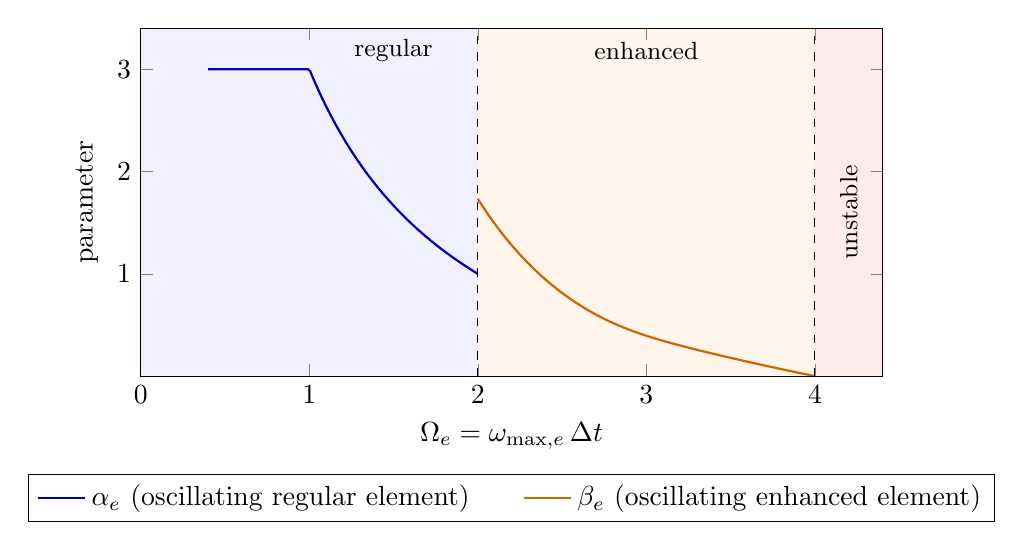
\begin{tikzpicture}
  \begin{axis}[
      width=11cm, height=6cm,
      xmin=0, xmax=4.4, ymin=0, ymax=3.4,
      xlabel={$\Omega_e=\omega_{\max,e}\,\Delta t$},
      ylabel={parameter},
      xtick={0,1,2,3,4}, ytick={1,2,3},
      legend style={at={(0.5,-0.28)}, anchor=north, legend columns=2,
                    /tikz/every even column/.append style={column sep=6mm}},
      legend cell align=left,
      every axis plot/.append style={thick},
      axis on top]
    % regions
    \fill[blue!6] (axis cs:0,0) rectangle (axis cs:2,3.4);
    \fill[orange!8] (axis cs:2,0) rectangle (axis cs:4,3.4);
    \fill[red!8] (axis cs:4,0) rectangle (axis cs:4.4,3.4);
    \node[font=\small] at (axis cs:1.5,3.18) {regular};
    \node[font=\small] at (axis cs:3,3.18) {enhanced};
    \node[font=\small, rotate=90] at (axis cs:4.2,1.6) {unstable};
    % alpha_e = min(3, 4/Omega - 1)
    \addplot[blue!70!black, domain=0.4:2, samples=120]
      {min(3, 4/x - 1)};
    \addlegendentry{$\alpha_e$ (oscillating regular element)}
    % beta_e
    \addplot[orange!80!black, domain=2.0001:4, samples=120]
      {(16 - (x^2-8)^2 + 4*sqrt(16 + 2*(x^2-8)^2))/x^4};
    \addlegendentry{$\beta_e$ (oscillating enhanced element)}
    \draw[dashed] (axis cs:2,0) -- (axis cs:2,3.4);
    \draw[dashed] (axis cs:4,0) -- (axis cs:4,3.4);
  \end{axis}
\end{tikzpicture}
